\section{Method}
\label{sec:method}
-Choosing have to divide the different datatypes into abstract representations
-Creating the syntax for the abstract representations
-checking the soundness of the abstract representations
-Creating the semantics for the abstract representations
-implementing the abstract representations in kotlin
-through CLI it takes a database in the form af SQL queries and returns the abstract representation of the database after a set of operations have been performed on it defined by the user
\todo{Clean this up}

\subsection{Example}\label{subsec:example}
To illustrate the method, we will use a simple example.
Consider a database with a single table, \texttt{account}, with two columns, \texttt{name} and \texttt{balance}.
For the program to work, we need to define the table for the database, this is shown in \autoref{lst:database-schema}.


\begin{listing}[htb!]
    \begin{minted}{sql}
    CREATE TABLE account (
        name    TEXT,
        balance INT
    );
    \end{minted}
    \caption{SQL query for creating the table in the database}
    \label{lst:database-schema}
\end{listing}


The database has two operations, \texttt{insert} and \texttt{update}.
The \texttt{insert} operation inserts a new row into the table, i.e.\ a new user, and the \texttt{update} operation updates the balance of two accounts.
The SQL queries for the operations are shown in \autoref{lst:sql-queries} and \autoref{lst:sql-queries2}.


\begin{listing}[htb!]
    \begin{minted}{sql}
        INSERT INTO account (name, balance)
        VALUES (RANDOM_NAME, RANDOM_AMOUNT);
    \end{minted}
    \caption{SQL query for the insert operation}
    \label{lst:sql-queries}
\end{listing}


\begin{listing}[htb!]
    \begin{minted}{SQL}
    UPDATE account
    SET balance = CASE
    WHEN name = "name1" THEN balance - <amount_to_transfer>
    WHEN name = "name2" THEN balance + <amount_to_transfer>
    ELSE balance
    END
    WHERE name IN (name1, name2);
    \end{minted}
    \caption{SQL query for the update operation}
    \label{lst:sql-queries2}
\end{listing}


Understanding the database schema and operations is crucial as it forms the foundation for defining the behavior of the operations.
The program that defines the behaviour of the operations is shown in \autoref{lst:program}.
The program first checks if there are two or more accounts in the database; if not, it inserts a new account with the \texttt{INSERT} operation.
If there are more than two accounts, we try to transfer an amount from one account to another; that is the \texttt{UPDATE} operation


\begin{listing}[htb!]
    \begin{minted}{bash}
transF || newuser

transF:
    transferAmount := ?
    formID := R_ID
    toID := R_ID
    if(transferAmount > 0)
        <select(fromB, id, DISTINCT(id(AccBalance)), true, id), toID = AccID>
        <select(toB, id, DISTINCT(id(AccBalance)), true, id), toID = AccID>
        <update(<AccBalance>, <fromB-transferAmount>), fromID = AccID>
        <update(<AccBalance>, <toB-transferAmount>), toID = AccID>

newuser:
    B := [0, +]
    U := ?
    <insert(U, B)> into (account)
    \end{minted}
    \caption{Program that defines the behavior of the operations}
    \label{lst:program}
\end{listing}


Now everything for the analysis is ready.
We just need to define what the analysis should check for.
This is defined by properties, which are defined by the LTL grammar on the attributes in the database.
The properties we want to check on the database are shown in \autoref{lst:properties}.

\begin{equation}
    \lozenge (transferAmount > 0)
    \label{eq:ltl-eventual-property}
\end{equation}


\begin{equation}
    \square (fromB-TransferAmount > 0)
    \label{eq:ltl-always-property}
\end{equation}


\begin{listing}[htb!]
    \begin{minted}{bash}
<>(transferAmount > 0)
[](fromB-TransferAmount > 0)
    \end{minted}
    \caption{Properties that the analysis check for}
    \label{lst:properties}
\end{listing}


After inserting all the information into the program, the program makes a graph of system, which is shown in \autoref{fig:program-graph}.

\begin{figure}
    \centering
    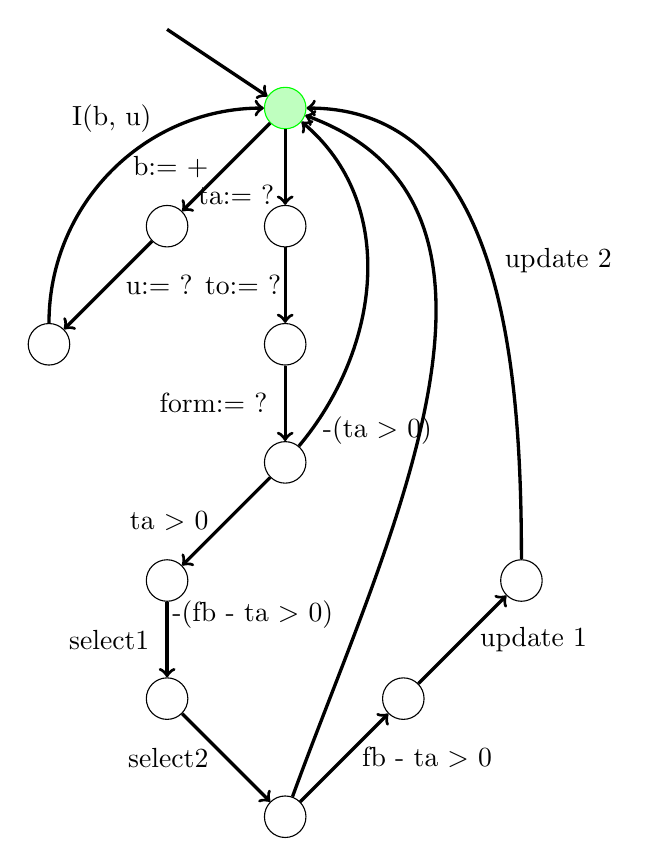
\begin{tikzpicture} [scale=0.5]
        \usetikzlibrary{arrows}
        \usetikzlibrary {shapes.geometric}
        \node (endState) [ellipse, draw, minimum size=1.5em] at (0,0) { }; \node (c1) [ellipse, draw, minimum size=1.5em] at (3,3) { };
        \node (c2) [ellipse, draw, minimum size=1.5em] at (6,6) { };
        \node (a5)[ellipse, draw, minimum size=1.5em] at (-3,3) { };
        \node (a4) [ellipse, draw, minimum size=1.5em] at (-3,6) { };
        \node (a3) [ellipse, draw, minimum size=1.5em] at (0,9) { };
        \node (a2) [ellipse, draw, minimum size=1.5em] at (0,12) { };
        \node (a1) [ellipse, draw, minimum size=1.5em] at (0,15) { };
        \node (b2) [ellipse, draw, minimum size=1.5em] at (-6,12) { };
        \node (b1) [ellipse, draw, minimum size=1.5em] at (-3,15) { };
        \node (startState) [ellipse, draw=green, fill=green!25, minimum size=1.5em] at (0,18) { };


        \draw [->, very thick]  (-3,20) to (startState);
        \draw [->, very thick] (startState) to node[midway, left=0.25em] {b:= +} (b1);
        \draw [->, very thick] (b1) to node[midway, right=0.25em] {u:= ?} (b2);
        \draw [->, very thick] (b2) to [out=90, in=180] node[midway, above=1em] {I(b, u)}  (startState);
        \draw [->, very thick] (startState) to node[midway, left=0em, yshift=-1em] {ta:= ?} (a1);
        \draw [->, very thick] (a1) to node[midway, left=0.25em, xshift=0.5em] {to:= ?} (a2);
        \draw [->, very thick] (a2) to node[midway, left=0.25em] {form:= ?} (a3);
        \draw [->, very thick] (a3) to [out=50, in=320] node[midway, right, xshift=-2em, yshift=-5.5em] {-(ta $>$ 0)} (startState);
        \draw [->, very thick] (a3) to node[midway, left=0.25em] {ta $>$ 0} (a4);
        \draw [->, very thick] (a4) to node[midway, left=0.25em] {select1} (a5);
        \draw [->, very thick] (a5) to node[midway, left=0.25em] {select2} (endState);
        \draw [->, very thick] (endState) to [out=70, in=340] node[midway, below left=3em, yshift=-4em] {-(fb - ta $>$ 0)} (startState);
        \draw [->, very thick] (endState) to node[midway, right=0.25em] {fb - ta $>$ 0} (c1);
        \draw [->, very thick] (c1) to node[midway, right=0.25em] {update 1} (c2);
        \draw [->, very thick] (c2) to [out=90, in=360] node[midway, right=0.25em] {update 2} (startState);
    \end{tikzpicture}
    \caption{Program graph for \autoref{lst:program}.}
    \label{fig:program-graph}
\end{figure}


The program is now ready to be analyzed, and the analysis will check if the properties are satisfied.


\begin{listing}[htb!]
    \begin{minted}{bash}
    Iteration 1:
        todo: {Initial state}
        state-space: {}

    Iteration 2:
        todo: {newuser}
        state-space: {}

    Iteration 3:
        todo: {newuser, newuser}
        state-space: {{}, {user1(R, [0, +])}}

    Iteration 4:
        todo: {{newuser, newuser, transF}, {newuser, newuser, newuser}}
        state-space: {{}, {user1(R, [0, +])}, {user1(R, [0, +]), user2(R, [0, +])}}

    Iteration 5:
        todo: {{newuser, newuser, newuser}, {newuser, newuser, transF, transF}}
        state-space: {{}, {user1(R, [0, +])}, {user1(R, [0, +]), user2(R, [0, +])}, {user1(R, [-, 0, +]), user2(R, [+])}}

    Iteration 6:
        todo: {newuser, newuser, transF, transF}
        state space: {{}, {user1(R, [0, +])}, {user1(R, [0, +]), user2(R, [0, +])}, {user1(R, [-, 0, +]), user2(R, [+])}, {user1(R, [0, +]), user2(R, [0, +]), user3(R, [0, +])}}

    STOP, no more states to explore
        Final state-space: {{}, {user1(R, [0, +])}, {user1(R, [0, +]), user2(R, [0, +])}, {user1(R, [-, 0, +]), user2(R, [+])}, {user1(R, [0, +]), user2(R, [0, +]), user3(R, [0, +])}, {user1(R, [+]), user2(R, [-, 0, +])}}
    \end{minted}
    \caption{Analysis of the example program}
    \label{lst:analysis}
\end{listing}


The analysis of the program is shown in \autoref{lst:analysis}.
Now that we have the whole state-space of the program, we can check if the properties are satisfied.
The first property is that the transfer amount is eventually greater than 0.
This is satisfied in the state-space, as the program checks if the transfer amount is greater than 0, and if not, it does not perform the transfer.

The second property is that the balance of the account from which the transfer is made is always greater than 0 after the transfer.
However, the second property, which states that the balance of the account that the transfer is made from is always greater than 0 after the transfer, is not satisfied in the state-space.
The program, unfortunately, does not check if the balance is greater than 0 after the transfer, only that the transfer amount is greater than 0.
Therefore, the second property is not satisfied.
This can be seen in the state-space, where the account balance is negative after the transfer.
